\section{Experiments}\label{sec:exp}

\paragraph{Setup.} We build two workflows from public intent-classification data
(details in Appendix~\ref{app:details}). \textbf{CLINC150}~\citep{larson2019clinc}: a
\texttt{scope} node separates in-scope from out-of-scope requests, a \texttt{domain} node
picks one of 10 product areas, and one \texttt{intent} node per area picks among its 15
intents: 12 decisions on a tree of depth 3 (Figure~\ref{fig:workflow}).
\textbf{MASSIVE}~\citep{fitzgerald2022massive} in four languages: a \texttt{language} node, a
\texttt{scenario} node per language (18 scenarios), and an \texttt{intent} node per scenario
that is shared by all languages: 21 decisions on a DAG with joins. Every node is a logistic
regression on frozen sentence embeddings~\citep{reimers2019sbert}, trained on the training
split; its confidence is the top class probability. Without abstention the workflows err on
\FreeErrClinc\% and \FreeErrMassive\% of inputs.

To measure validity without test-set noise we treat the pooled held-out data (8{,}600 and
20{,}028 inputs) as the population: a calibration set is $n$ i.i.d.\ draws from it, and each
selected threshold vector is scored by its exact risk and review rate on the population. We
report means over repeated draws and the \emph{violation rate}, the fraction of draws whose
population risk exceeds $\eps$; a method with a $(1-\delta)$ guarantee must keep it below
$\delta=0.1$.

\paragraph{Methods.} Without guarantee: a fixed threshold of 0.7; \emph{per-node selective
risk}, which tunes each node separately so that its own error rate among committed inputs is
certified below $\eps$; and a \emph{plug-in} version of our certificate without confidence
bounds. End to end, valid for one pre-specified target: a single \emph{shared threshold}
calibrated by fixed-sequence testing on the exact risk~\citep{angelopoulos2021ltt}, the
selective-risk counterpart of joint-score calibration~\citep{ren2023knowno,kotte2026pasc}; and
\emph{Pareto testing}~\citep{laufer2022pareto} over per-node thresholds, with half of the
data proposing candidates and half testing them. Uniform over the grid: an \emph{end-to-end
uniform} bound on the exact error count with the same union as Theorem~\ref{thm:cert}; and
our certificates with TF, FE and LC charging, with modules per node, per level, or shared.

\subsection{Validity and efficiency}\label{sec:exp-main}

\begin{table}[t]
\centering\footnotesize
\setlength{\tabcolsep}{3.5pt}
\begin{tabular}{llrrrrrrrrr}
\toprule
 & & \multicolumn{3}{c}{$\varepsilon=2\%$} & \multicolumn{3}{c}{$\varepsilon=5\%$} & \multicolumn{3}{c}{$\varepsilon=10\%$} \\
\cmidrule(lr){3-5}\cmidrule(lr){6-8}\cmidrule(lr){9-11}
Method & Guarantee & viol. & risk & review & viol. & risk & review & viol. & risk & review \\
\midrule
Fixed threshold 0.7 & none & 100 & 4.6 & 22.5 & 0 & 4.6 & 22.5 & 0 & 4.6 & 22.5 \\
Per-node selective risk & none & 0 & 0.0 & 100.0 & 0 & 1.7 & 76.6 & 100 & 12.3 & 10.1 \\
Plug-in (no confidence bound) & none & 68 & 2.1 & 37.0 & 64 & 5.1 & 20.4 & 54 & 10.0 & 8.3 \\
\midrule
Shared threshold, end-to-end LTT & fixed & 1 & 1.4 & 53.1 & 0 & 4.1 & 25.2 & 0 & 8.6 & 11.6 \\
End-to-end Pareto testing & fixed & 2 & 1.4 & 49.9 & 3 & 4.1 & 25.0 & 3 & 8.6 & 11.6 \\
End-to-end, uniform over grid & uniform & 0 & 0.6 & 67.7 & 0 & 2.4 & 36.4 & 0 & 6.2 & 17.8 \\
\midrule
Teacher-forced, per node & uniform & 0 & 0.0 & 100.0 & 0 & 0.2 & 87.2 & 0 & 2.5 & 41.1 \\
First-error, per node & uniform & 0 & 0.0 & 100.0 & 0 & 0.7 & 73.9 & 0 & 3.9 & 36.6 \\
First-error, per level & uniform & 0 & 0.0 & 99.4 & 0 & 0.9 & 58.9 & 0 & 5.8 & 30.1 \\
\midrule
Least-confident, per node & uniform & 0 & 0.5 & 64.7 & 0 & 2.4 & 34.3 & 0 & 6.2 & 17.4 \\
Least-confident, per level & uniform & 0 & 1.0 & 50.3 & 0 & 3.4 & 27.8 & 0 & 7.8 & 13.6 \\
Least-confident, shared & uniform & 0 & 1.1 & 61.4 & 0 & 3.7 & 27.1 & 0 & 8.1 & 12.8 \\
Anchored, per level & uniform & 0 & 0.7 & 61.6 & 0 & 3.1 & 29.7 & 0 & 7.3 & 14.7 \\
\bottomrule
\end{tabular}

\caption{CLINC150, $n=4{,}000$, $\delta=0.1$, \Trials\ calibration draws. \emph{viol.}:
percentage of draws with population risk above $\eps$ (bold: above $\delta$ for a method
that claims a guarantee); \emph{risk}, \emph{review}: mean population risk and human review
rate in percent. ``fixed'': valid for the single target it was run for; ``uniform'': valid
for all thresholds on the grid at once.}\label{tab:main}
\end{table}

Table~\ref{tab:main} gives the results for CLINC150 and Table~\ref{tab:main-massive} in the
appendix for MASSIVE.

\paragraph{Uncertified practice fails where it matters.} Per-node selective calibration
controls each node's own error rate and ignores that errors accumulate along a route: at
$\eps=10\%$ it exceeds the target in \ViolCPerNodeTen\% of draws on CLINC150 and
\ViolMPerNodeTen\% on MASSIVE. The plug-in certificate, which uses frequencies in place of
confidence bounds, violates in \ViolCPlugFive\% and \ViolMPlugFive\% of draws at $\eps=5\%$.
Every method with a guarantee stays within $\delta$: the largest violation rate among them, over both workflows and
all targets, is \MaxViolCertified\%.

\paragraph{The rescue effect.} FE and TF certificates are valid but nearly useless on
CLINC150: at $\eps=5\%$ they escalate \RevCFEnodeFive\% and \RevCTFnodeFive\% of inputs, against
\RevCLCnodeFive\% for LC with the same per-node modules and the same union bound. The reason is
visible in the population. At the thresholds chosen by the shared end-to-end method for
$\eps=5\%$, the mass of deviating runs whose first wrong node commits is \FdMassC\%, while the
actual risk is \RiskCSharedFive\%: \RescuedShareC\% of the first-error mass is escalated
further along the route. The \texttt{scope} node passes out-of-scope requests with high
confidence, and the \texttt{domain} and \texttt{intent} nodes, facing inputs unlike anything
they were trained on, hesitate. On MASSIVE, where errors are spread over more nodes, the
first-error mass still overstates the risk by a factor of \FdRatioM\ (\RescuedShareM\%
rescued), and FE needs \RevMFEnodeFive\% review where LC needs \RevMLCnodeFive\%. Additive
attribution to the causing stage, which is exact for a cascade of interchangeable solvers,
therefore misjudges routing workflows.

\paragraph{The price of uniformity and of granularity.} Among the certified methods, Pareto
testing escalates least at a fixed target (\RevCParetoFive\% on CLINC150 and
\RevMParetoFive\% on MASSIVE at $\eps=5\%$), as it tests a short pre-ordered list of
configurations and pays no union over the grid. Certificates that stay valid under retuning
pay for it: LC per level needs \RevCLClevelFive\% and \RevMLClevelFive\%, LC per node
\RevCLCnodeFive\% and \RevMLCnodeFive\%. The separable bound is not the bottleneck: the
end-to-end uniform bound, which uses exact error counts and the same union, needs
\RevCUnifFive\% and \RevMUnifFive\%, no less than LC per node, because its feasible set can
only be searched heuristically whereas the separable problem is solved exactly. With a single
shared module the LC certificate uses exactly the end-to-end error counts
(Proposition~\ref{prop:exact}); its remaining distance to the shared-threshold baseline
(\RevCLCsharedFive\% against \RevCSharedFive\%) is the union over the grid. How much there is
to gain from per-node thresholds depends on the workflow: with thresholds optimised directly
on the population, per-node thresholds reach $\eps=5\%$ at \OracleNodeCFive\% review against
\OracleSharedCFive\% for the best shared threshold on CLINC150, and \OracleNodeMFive\% against
\OracleSharedMFive\% on MASSIVE. Tying thresholds by level is a good default: it keeps most of
the control and pays the union for three modules only.

\subsection{Calibration size and number of decisions}

\begin{figure}[t]
\centering
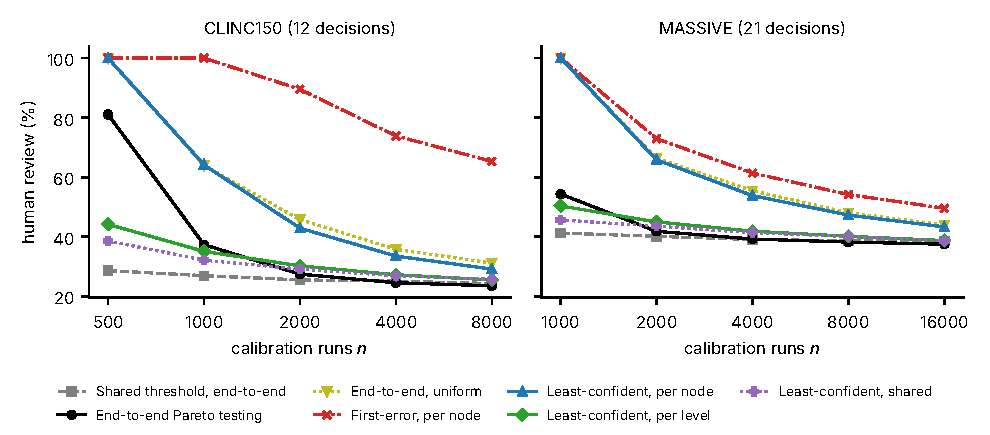
\includegraphics[width=\linewidth]{figures/nsweep.pdf}
\caption{Human review needed to certify $\eps=5\%$ as a function of the calibration size
(\NsweepTrials\ draws per point, $\delta=0.1$).}\label{fig:nsweep}
\end{figure}

\begin{figure}[t]
\centering
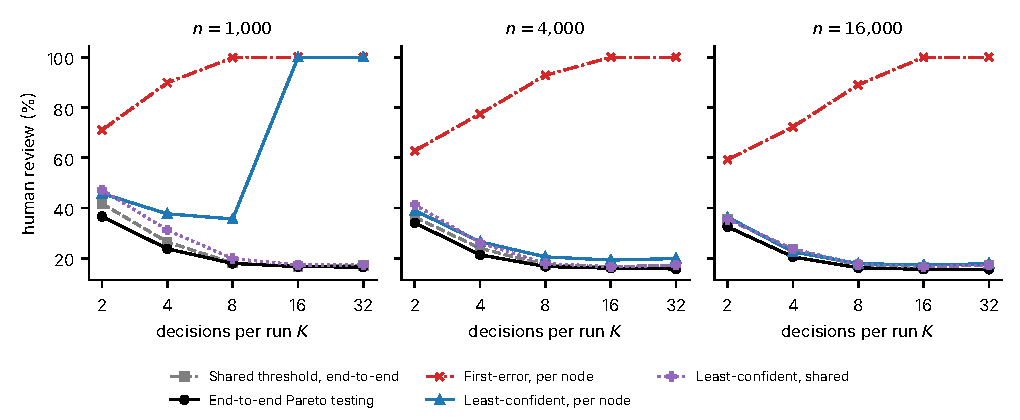
\includegraphics[width=\linewidth]{figures/synth.pdf}
\caption{Synthetic chains of $K$ decisions with 20\% erroneous runs before abstention:
review needed to certify $\eps=5\%$ (\SynthTrials\ draws per point). The per-node certificate
pays a union over $K$ thresholds; a shared module does not.}\label{fig:synth}
\end{figure}

Figure~\ref{fig:nsweep} varies $n$. The gap between uniform and fixed-target methods is a
statistical margin and closes as $n$ grows; with few calibration runs, fine-grained uniform
certificates cannot certify at all, and the shared and per-level variants degrade most
gracefully. Figure~\ref{fig:synth} isolates the dependence on the number of decisions with
synthetic chains in which every run visits all $K$ nodes, node errors are correlated through
a shared difficulty, and confidences are overconfident. The per-node certificate needs
\SynthTwoSmallLCnode\% review for $K=2$ and \SynthThirtyTwoSmallLCnode\% for $K=32$ at
$n=1{,}000$, and \SynthTwoLargeLCnode\% and \SynthThirtyTwoLargeLCnode\% at $n=16{,}000$,
consistent with a margin of order $K\ln G/n$; the shared module is insensitive to $K$. FE
charging is loose throughout because the chains have rescue by construction.

\subsection{Post hoc retuning}

\begin{figure}[t]
\centering
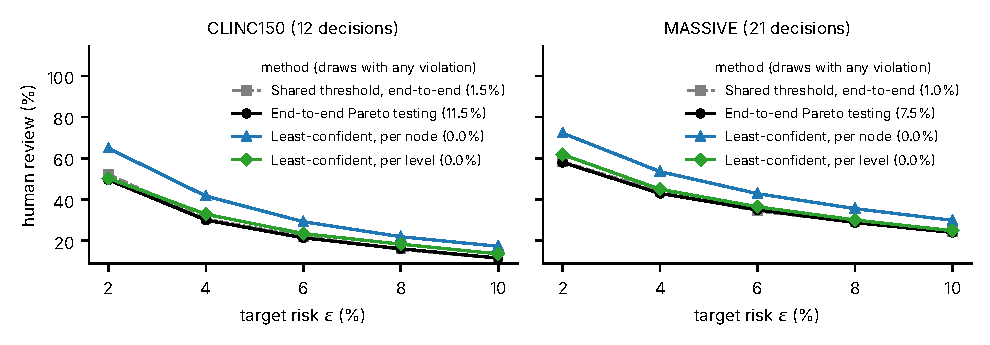
\includegraphics[width=\linewidth]{figures/posthoc.pdf}
\caption{One calibration set, five targets. The LC certificates are issued once and
re-optimised for each $\eps$; the end-to-end procedures are re-run for each $\eps$ on the same
data. In parentheses: percentage of calibration draws in which at least one of the five
selected configurations violates its target (\PosthocTrials\ draws).}\label{fig:posthoc}
\end{figure}

Operators rarely keep one target. Figure~\ref{fig:posthoc} issues a certificate once and then
selects thresholds for five targets from 2\% to 10\%. For the LC certificates this is covered
by Corollary~\ref{cor:posthoc}: in \AnyViolCLClevel\% (CLINC150) and \AnyViolMLClevel\%
(MASSIVE) of draws at least one of the five configurations violates its target. Re-running
an end-to-end procedure for each target on the same data is not covered by its guarantee.
In our experiments the simultaneous violation rates of the re-run procedures are
\AnyViolCPareto\% and \AnyViolMPareto\% for Pareto testing and \AnyViolCShared\% and
\AnyViolMShared\% for the shared threshold; the selected configurations are strongly
dependent across targets, so the inflation over the per-target level is modest here, but
nothing bounds it in general.

\subsection{Edits}\label{sec:exp-edits}

\begin{figure}[t]
\centering
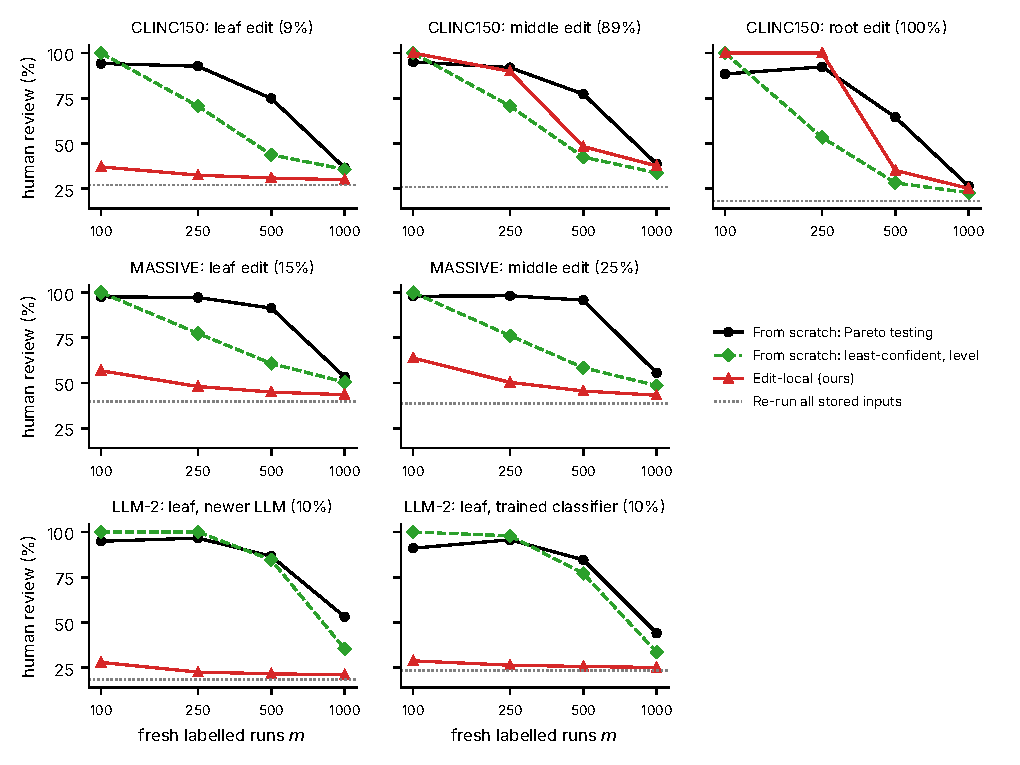
\includegraphics[width=\linewidth]{figures/edits.pdf}
\caption{Review needed to certify $\eps=5\%$ after replacing the model of one node, as a
function of the number $m$ of fresh labelled runs (\EditTrials\ draws per point). \emph{From
scratch} labels $m$ runs of all traffic and recalibrates with them alone. \emph{Edit-local}
(Theorem~\ref{thm:recert}) keeps the old certificate for the routes that avoid the node and
labels $m$ runs of the traffic through it. The dotted line recalibrates on all stored inputs
re-run through the edited workflow, which assumes they were kept.}\label{fig:edits}
\end{figure}

We replace the model of one node by a model from a different family and ask how many fresh
labels are needed to certify the edited workflow at $\eps=5\%$ (Figure~\ref{fig:edits}). The
old certificate was issued from $n$ runs of the unedited workflow. We first confirmed
Proposition~\ref{prop:local} on the populations: for each edit, the runs that avoid the
edited node have identical routes, confidences and deviation status before and after.

For a leaf (\EditShareCLeaf\% of the traffic on CLINC150, \EditShareMLeaf\% on MASSIVE) the
edit-local certificate needs \EditCLeafLocalHundred\% and \EditMLeafLocalHundred\% review with
$m=100$ fresh labels. Recalibrating from scratch with 100 labels certifies nothing
(\EditCLeafScratchHundred\% and \EditMLeafScratchHundred\% review with Pareto testing), and
with $m=1{,}000$ it reaches \EditCLeafScratchThousand\% and \EditMLeafScratchThousand\%, where
the edit-local certificate is at \EditCLeafLocalThousand\% and \EditMLeafLocalThousand\%. For a
middle node the picture depends on its traffic share: a \texttt{scenario} node of MASSIVE
(\EditShareMMiddle\% of the traffic) is repaired locally with 100 labels at
\EditMMiddleLocalHundred\% review, while the \texttt{domain} node of CLINC150 carries
\EditShareCMiddle\% of the traffic, leaves little to reuse, and gains nothing from
locality. Editing the root touches every run, and the edit-local procedure then reduces to
recalibration from scratch with a smaller share of $\delta$. Across all edits and sample sizes
the largest violation rate of the edit-local certificates is \EditMaxViolLocal\%.

If all calibration inputs and labels were retained, re-running them through the edited
workflow and recalibrating is at least as good (dotted line); that option requires storing
raw inputs, and each such recalibration is a new certificate for a single configuration. The
edit-local certificate needs only the stored counts.
